\documentclass{article}

\usepackage{titlesec}
\usepackage{pgf-umlcd}
\newcommand{\sectionbreak}{\clearpage}

\begin{document}

\begin{titlepage}
	\Huge{Assignment 1}
\end{titlepage}


\section{The Core}

\subsection{Derive Classes}

The following list of classes can be derived from the requirements document\footnote{https://github.com/mkhattat/bitcode-SEM/blob/master/docs/requirements.pdf}.


\subsection{Main Classes}
text

\subsection{Reflect on main class decisions}
text

\subsection{The Class diagram}
text

\subsection{The Sequence Diagram}
text




\section{UML in Practice}
text

\subsection{Composition and Aggregation}
text

\subsection{Parametrized Classes}
text

\subsection{Hierarchy Class Diagrams}
\centering
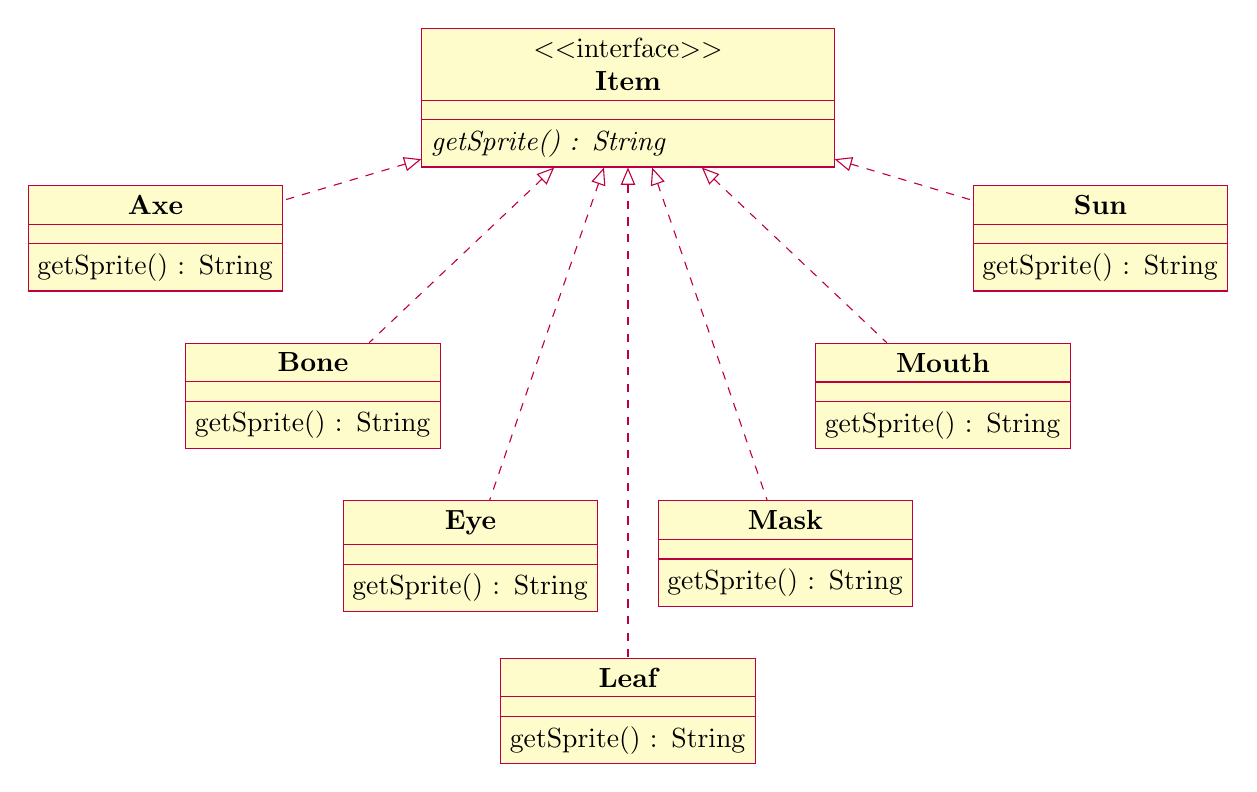
\begin{tikzpicture}
\begin{interface}{Item}{0,0}
\operation[0]{getSprite() : String}
\end{interface}
\begin{class}[text width = 3cm]{Axe}{-6,-2}
\implement{Item}
\operation{getSprite() : String}
\end{class}
\begin{class}[text width = 3cm]{Bone}{-4,-4}
\implement{Item}
\operation{getSprite() : String}
\end{class}
\begin{class}[text width = 3cm]{Eye}{-2,-6}
\implement{Item}
\operation{getSprite() : String}
\end{class}
\begin{class}[text width = 3cm]{Leaf}{0,-8}
\implement{Item}
\operation{getSprite() : String}
\end{class}
\begin{class}[text width = 3cm]{Mask}{2,-6}
\implement{Item}
\operation{getSprite() : String}
\end{class}
\begin{class}[text width = 3cm]{Mouth}{4,-4}
\implement{Item}
\operation{getSprite() : String}
\end{class}
\begin{class}[text width = 3cm]{Sun}{6,-2}
\implement{Item}
\operation{getSprite() : String}
\end{class}
\end{tikzpicture}

Items are produced by an item factory, which can create each of the seven types of items.
Each item implements the item interface, as a result the board can contain every type of item and request its sprite.
A similar functionality could be implemented using an item class with an id attribute, however such an implementation would make further expanding each item individually much more complicated and inconvenient.


\centering
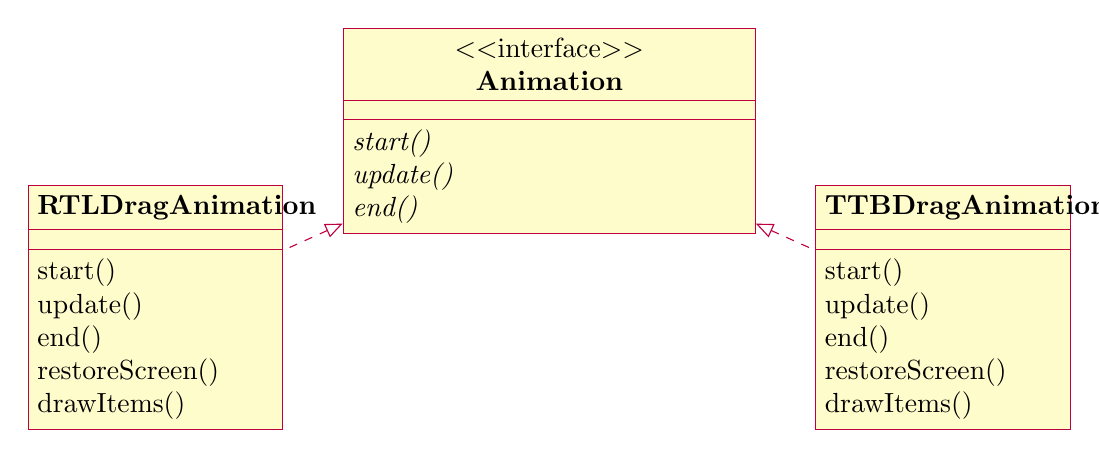
\begin{tikzpicture}
\begin{interface}{Animation}{0,0}
\operation[0]{start()}
\operation[0]{update()}
\operation[0]{end()}
\end{interface}
\begin{class}[text width = 3cm]{RTLDragAnimation}{-5,-2}
\implement{Animation}
\operation{start()}
\operation{update()}
\operation{end()}
\operation{restoreScreen()}
\operation{drawItems()}
\end{class}
\begin{class}[text width = 3cm]{TTBDragAnimation}{5,-2}
\implement{Animation}
\operation{start()}
\operation{update()}
\operation{end()}
\operation{restoreScreen()}
\operation{drawItems()}
\end{class}
\end{tikzpicture}

This hierarchy generalizes the behavior of animations, making it easier to work with different animations.

Furthermore, the MouseEventHandler class implements the MouseListener and MouseMotionListener interfaces from the java.awt.event library so it can handle mouse events.
The MainScreen class and the JPanelTile class extend the JLayeredPane class and the JPane class, respectively; Both of these superclasses are from the javax.swing library and are used to create a UI.


\end{document}

